 \documentclass[a4paper, 11pt]{article}

%%%%%% 导入包 %%%%%%
\usepackage{CJKutf8}
\usepackage{graphicx}
\usepackage[unicode]{hyperref}
\usepackage{xcolor}
\usepackage{color}
\usepackage{cite}
\usepackage{indentfirst}
\usepackage{tikz,mathpazo}
\usetikzlibrary{shapes.geometric, arrows}
%%%%%% 设置字号 %%%%%%
\newcommand{\chuhao}{\fontsize{42pt}{\baselineskip}\selectfont}
\newcommand{\xiaochuhao}{\fontsize{36pt}{\baselineskip}\selectfont}
\newcommand{\yihao}{\fontsize{28pt}{\baselineskip}\selectfont}
\newcommand{\erhao}{\fontsize{21pt}{\baselineskip}\selectfont}
\newcommand{\xiaoerhao}{\fontsize{18pt}{\baselineskip}\selectfont}
\newcommand{\sanhao}{\fontsize{15.75pt}{\baselineskip}\selectfont}
\newcommand{\sihao}{\fontsize{14pt}{\baselineskip}\selectfont}
\newcommand{\xiaosihao}{\fontsize{12pt}{\baselineskip}\selectfont}
\newcommand{\wuhao}{\fontsize{10.5pt}{\baselineskip}\selectfont}
\newcommand{\xiaowuhao}{\fontsize{9pt}{\baselineskip}\selectfont}
\newcommand{\liuhao}{\fontsize{7.875pt}{\baselineskip}\selectfont}
\newcommand{\qihao}{\fontsize{5.25pt}{\baselineskip}\selectfont}

%%%% 设置 section 属性 %%%%
\makeatletter
\renewcommand\section{\@startsection{section}{1}{\z@}%
{-1.5ex \@plus -.5ex \@minus -.2ex}%
{.5ex \@plus .1ex}%
{\normalfont\sihao\CJKfamily{hei}}}
\makeatother

%%%% 设置 subsection 属性 %%%%
\makeatletter
\renewcommand\subsection{\@startsection{subsection}{1}{\z@}%
{-1.25ex \@plus -.5ex \@minus -.2ex}%
{.4ex \@plus .1ex}%
{\normalfont\xiaosihao\CJKfamily{hei}}}
\makeatother

%%%% 设置 subsubsection 属性 %%%%
\makeatletter
\renewcommand\subsubsection{\@startsection{subsubsection}{1}{\z@}%
{-1ex \@plus -.5ex \@minus -.2ex}%
{.3ex \@plus .1ex}%
{\normalfont\xiaosihao\CJKfamily{hei}}}
\makeatother

%%%% 段落首行缩进两个字 %%%%
\makeatletter
\let\@afterindentfalse\@afterindenttrue
\@afterindenttrue
\makeatother
\setlength{\parindent}{2em}  %中文缩进两个汉字位


%%%% 下面的命令重定义页面边距,使其符合中文刊物习惯 %%%%
\addtolength{\topmargin}{-54pt}
\setlength{\oddsidemargin}{0.63cm}  % 3.17cm - 1 inch
\setlength{\evensidemargin}{\oddsidemargin}
\setlength{\textwidth}{14.66cm}
\setlength{\textheight}{24.00cm}    % 24.62

%%%% 下面的命令设置行间距与段落间距 %%%%
\linespread{1.4}
% \setlength{\parskip}{1ex}
\setlength{\parskip}{0.5\baselineskip}

%%%% 正文开始 %%%%
\begin{document}
\begin{CJK}{UTF8}{gbsn}

%%%% 定理类环境的定义 %%%%
\newtheorem{example}{例}             % 整体编号
\newtheorem{algorithm}{算法}
\newtheorem{theorem}{定理}[section]  % 按 section 编号
\newtheorem{definition}{定义}
\newtheorem{axiom}{公理}
\newtheorem{property}{性质}
\newtheorem{proposition}{命题}
\newtheorem{lemma}{引理}
\newtheorem{corollary}{推论}
\newtheorem{remark}{注解}
\newtheorem{condition}{条件}
\newtheorem{conclusion}{结论}
\newtheorem{assumption}{假设}




%%%% 定义标题格式,包括title,author,affiliation,email等 %%%%
\title{ 阅读论文综述}
\author{王俊杰\footnote{电子邮件: wangjunjie2013@gmail.com}\\[2ex]
\xiaosihao 哈尔滨工业大学\\[2ex]
}
\date{}


%%%% 以下部分是正文 %%%%
\maketitle


 \begin{tabular}{|c|ccccccccccc|}
\hline
正体&$\Gamma$ & $\Delta$ & $\Theta$ & $\Lambda$ & $\Xi$ & $\Pi$ & $\Sigma$ & $\Upsilon$ & $\Phi$ & $\Psi$ & $\Omega$\\
\hline
\verb|\mit|斜体&$\mit\Gamma$ & $\mit\Delta$ & $\mit\Theta$ & $\mit\Lambda$ & $\mit\Xi$ & $\mit\Pi$ & $\mit\Sigma$ &  $\mit\Upsilon$ & $\mit\Phi$ & $\mit\Psi$ & $\mit\Omega$\\
\hline
\end{tabular}


 \begin{tabular}{|lcc|lcc|}
\hline
命令 & 大写 & 小写 & 命令 & 大写 & 小写 \\
\hline
  alpha & $A$ & $\alpha$ &  beta & $B$ &$\beta$  \\
  gamma & $\Gamma$ & $\gamma$  &  delta & $\Delta$ & $\delta$ \\
  epsilon & $E$ & $\epsilon,\varepsilon$ &  zeta & $Z$ & $\zeta$ \\
   eta & $H$ &$\eta$  &  theta & $\Theta$ & $\theta,\vartheta$ \\
  iota & $I$ & $\iota$ &   kappa & $K$ & $\kappa$ \\
  lambda & $\Lambda$ & $\lambda$  & mu & $M$ & $\mu$ \\
  nu & $N$ & $\nu$ & omicron & $O$ & $o$ \\
    xi & $\Xi$ & $\xi$  &   pi & $\Pi$ & $\pi,\varpi$ \\
    rho & $P$ & $\rho,\varrho$  &  sigma & $\Sigma$ & $\sigma,\varsigma$ \\
   tau & $T$ & $\tau$ &   upsilon & $\Upsilon$ & $\upsilon$ \\
  phi & $\Phi$ & $\phi,\varphi$ &  chi & $X$ & $\chi$ \\
  psi & $\Psi$ & $\psi$  &  omega & $\Omega$ &$\omega$ \\
\hline
\end{tabular}


\newpage
\tableofcontents
\newpage

\section{AVERAGE CONSENSUS-BASED ASYNCHRONOUS TRACKING}
Target tracking in a network may fail if data are captured or exchanged asynchronously. Most distributed tracking algorithms assume that the cameras in the network capture the frames synchronously. In this paper, we propose an Average Consensus-based Asynchronous tracking Filter(ACAF) for WCNs. The nodes perform time-alignment with respect to their capturing instant by predicting the information of the neighbours. Each node performs iteratively two phases, namely estimation and fusion. The fusion phase exchanges, aligns and fuses the local pdfs. The expected pdf of the sending node is estimated by a receiving node with a time reversed prediction. The nodes discard the pdfs received before the frame capture and terminate their fusion phase before any other node captures the next frame.

\begin{figure}[!htp]
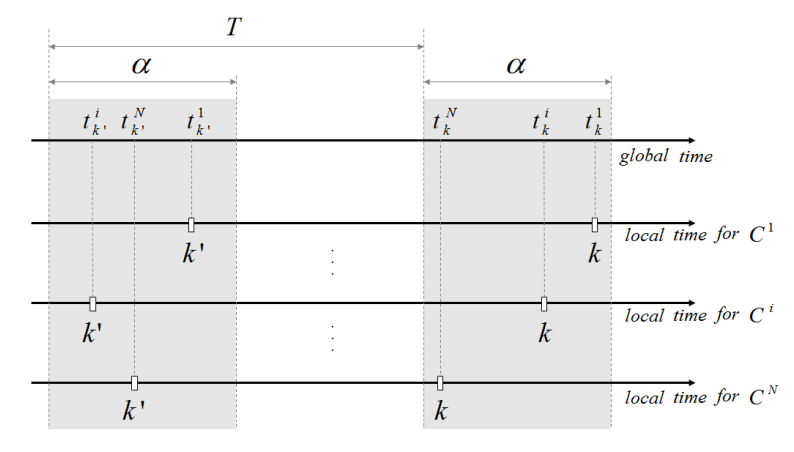
\includegraphics[scale=0.5]{image/07/localandglobalclocks.png}
\caption{Local and global clocks in partial asynchronism. The vertical grey stripes associate the local time instants }
\end{figure}
Let $t_k^i$ be the global-clock time whrn the local clock time of $C^i$ is $k$ and $T$ be the desired inter-frame capturing period for all cameras. In the synchronous case, $t_k^i = k$, and the camers capture frames at $0,T,2T...$. In the asynchronous case, the cameras capure frames at different instants.

\subsection{Prediction and Fusion}
At the beginning of the fusion phase, each node $C^i$ performs three predictions.

\textbf{backward prediction} The first predictis the target pdf for $k-\alpha$ based on the computed local pdf $f(x_k^i|z_{1:k}^i)$.

\textbf{forward prediction} The second prediction is based on the previous known pdf $f(\hat{x}_{k^{''}}^i | z_{1:k^{'}}^i)$. The predicted pdfs are then compared and the one with lowest uncertainty is considered.

\textbf{forward prediction} The third predicts the pdf for the capturing instant $k$ based on the certain predicted pdf corresponding to $k-\alpha$ based on certain predicted pdf corresponding to $k-\alpha$


\end{CJK}
\end{document}